\begin{quote}
    Game: A competitive activity involving skill, chance, or endurance on the part of two or more persons who play according to a set of rules, usually for their own amusement or for that of spectators.\\
\end{quote}
\begin{figure}
    \centering
    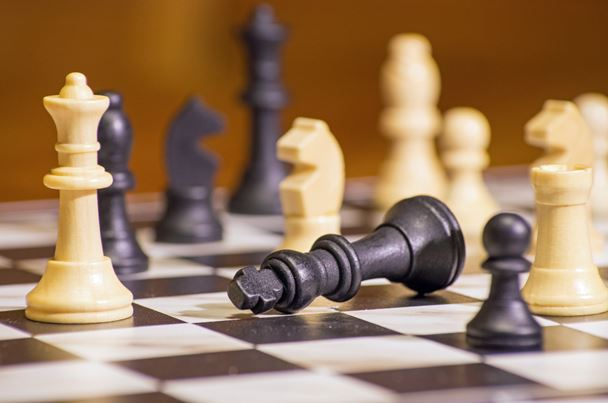
\includegraphics[]{game.jpg}
    \caption{gametheory}\\
    Source: https://cdn.static-economist.com/sites/default/
    \label{game:1}
\end{figure}
After learning how to play the game tick-tack-toe, you probably discovered a strategy of play that enables you to achieve at least a draw and even win if your opponent makes a mistake and you notice it. Sticking to that strategy ensures that you will not lose.

This simple game illustrates the essential aspects of what is now called game theory. In it, a game is the set of rules that describe it. An instance of the game from beginning to end is known as a play of the game. And a pure strategy--such as the one you found for tick-tack-toe--is an overall plan specifying moves to be taken in all eventualities that can arise in a play of the game. A game is said to have perfect information if, throughout its play, all the rules, possible choices, and past history of play by any player are known to all participants. Games like tick-tack-toe, backgammon and chess are games with perfect information and such games are solved by pure strategies. But whereas you may be able to describe all such pure strategies for tick-tack-toe, it is not possible to do so for chess, hence the latter's age-old intrigue.


A game has the following
\begin{table}[h!]
  \begin{center}
    \caption{Components}
    \label{tab:table1}
    \begin{tabular}{l|S|r}
      \hline
    Set of Players & $\mathrm { D } = \left\{\mathrm {P}_{\mathrm{i }}|1<=\mathrm{i}<=\mathrm{n}\right\}$\\
      Set of rules & R \\
      Set of Strategies & $\mathrm { S } _ { \mathrm {i} } \text { for each player } \mathrm { P } _ { \mathrm { i } }$ \\
      Set of Outcomes & O\\
      Pay off & u for each outcome
    \end{tabular}
  \end{center}
\end{table}
